\chapter{New association measure}

Natural Language Processing is developing very quickly nowadays, but extraction of collocations is still quite low advanced field \cite{ramisch}. 
In the recent years a couple of papers and books have been published in this topic, but most of them describes method for extraction of MWE in English 
and since this task is strongly language dependent, polish literature about this subject is much more valuable for this thesis.
In 2016 Polish scientists published paper about their application for polish terminology extraction \cite{termopl}. 
Method that they use for that task is very similar to described in section \ref{extraction_method}. 
Whole extraction is a 3-stage process. At first candidates for terms are selected from text basing on grammar rules. 
Second step is evaluation of candidates using term quality measure and making ranking accordingly to the obtained score. 
Final step is filtering out general terms used in many domains by comparing phrases containing that terms to those obtained from non-domain corpora.
Principle of working is similar to the one used in MeWeX, also definition of terminology used in that paper 
partially cover definition of collocation used in this thesis. The difference is, that in opposition to MWE, term can be a single word, 
also terminology is domain-specific only while collocation can be also noncompositional general expression. 
These discrepancies may be easily walk around by adding some simple constraints and then the same method can be used for extracting MWE. 
First stage of processing is very similar to already implemented, so this can be skipped. Last one filters out general terms, 
which is not desired step in collocation extraction. Middle stage uses quality measure to evaluate candidates and sort them 
accordingly to the obtained score, but TermoPL uses for that purpose C-value measure, which is not implemented in MeWeX. 
Extending available list of association measures by this new function can improve efficiency of the system.

\section{C-Value}
Most significant factor in C-value is frequency of given phrase what is a common practice in association measures. 
Longer tuples are less frequent, so multiplying by logarithm of tuple length reduces that disadvantage. 
The most distinctive part from other measures is subtracting frequencies of all tuples containing given phrase divided by number of those tuples. 
This part decreases score for candidates which occure often in different context.
\clearpage
\[ 
    C{\text -}value(p) = \begin{cases}
        l(p) * (freq(p) - \frac{1}{r(LP)}\sum_{lp \in LP}{freq(lp)}) & \text{if } r(LP) > 0\\
        l(p) * freq(p)            & \text{if } r(LP) = 0\\
    \end{cases}
\]
Where: \\
\(p\)  - phrase \\
\(l(p) = ln(length(p))\) \\
\(LP\)  - set of phrases containing \(p\) \\
\(r(LP)\) - number of elements of \(LP\) \\

This function was modified in relation to the one used in TermoPL. In original measure, function \(l(p) = ln(length(p)) + C\) 
contained also constant, because it was based on assumption that length of \(p\) can be equal to 1. This constant was removed 
from formula as it became redundant for MWE.

\subsection{Motivation}
MeWeX contains many association measure which base on frequency, expected frequency, order, number of relation etc. 
and using vector association measure it can make an advantage of all those features at once. That leads to assumption that adding new measure, 
which values properties not considered before, should increase quality of result. C-value base on frequency and length of phrase, 
but also it takes into account number of different contexts it takes. This property is not covered by any other already implemented function.
Measure W Order is quite similar, but this one checks only number of other relations in which given tuples occurred, 
while C-value also accounts tuples which contains given phrase and measures also frequency.

\clearpage
\subsection{Measure implementation}
Expanded structure and modular architecture of MeWeX made simple further extensions of code. To implement new association 
it was necesary to create new class that inherits class \textit{AssociationFunction}.
\vspace{1em}
\begin{lstlisting}
#include "AssociationFunction.h"

namespace function
{
    namespace association
    {

class Cvalue : public AssociationFunction
{
public:
    virtual AssociationMeasurePtrS copy() const override;

    virtual double rankUsingTable(
        TupleId pTupleId,
        ContingencyTable const& pContingencyTable) const override;

    virtual std::string	name() const override;
};

    }
}
\end{lstlisting}
\vspace{1em}
Then, to make it possible to choose that measure in other modules or programs, name of that function had to be added to the mapping,
that maps name to specific function.
\vspace{1em}
\begin{lstlisting}
Creators::FunctionMapping const AssociationFunctionCreators::MAPPING(
{
    ...

    {"c_value",     &Cvalue},
    {"cval",        &Cvalue},

    ...
});
\end{lstlisting}
\clearpage
And last step was to implement the function itself.
\vspace{1em}
\begin{lstlisting}
double Cvalue::rankUsingTable(
                    TupleId pTupleId, 
                    ContingencyTable const& pContingencyTable) const
{
    double LP = 0.0, LPsum = 0.0;
    for(int i = 1; i < pContingencyTable.size() - 1;i++)
    {
        LPsum += pContingencyTable[i].observed;
        if(pContingencyTable[i].observed > 0)
            LP += 1.0;
    }
    double l = log(pContingencyTable.tupleSize());

    if(LP == 0)
    {
        return (l * pContingencyTable[0].observed);
    }
    else
    {
        return (l * (pContingencyTable[0].observed - (LPsum/LP)));
    }
}
\end{lstlisting}
\clearpage

\subsection{Quality evaluation}
In the figure \ref{img_cval} are presented exemplary results obtained with use of C-value association measure. 
It is hard to manually evaluate quality of all results but in top 50 tuples from k-best list almost all suits the definition of collocation, 
so that is satisfactionary score. More precise evaluation, quality of this measure, method and setup for verification 
is described in chapter \ref{verification}.
\begin{figure}[ht]
    \centering
    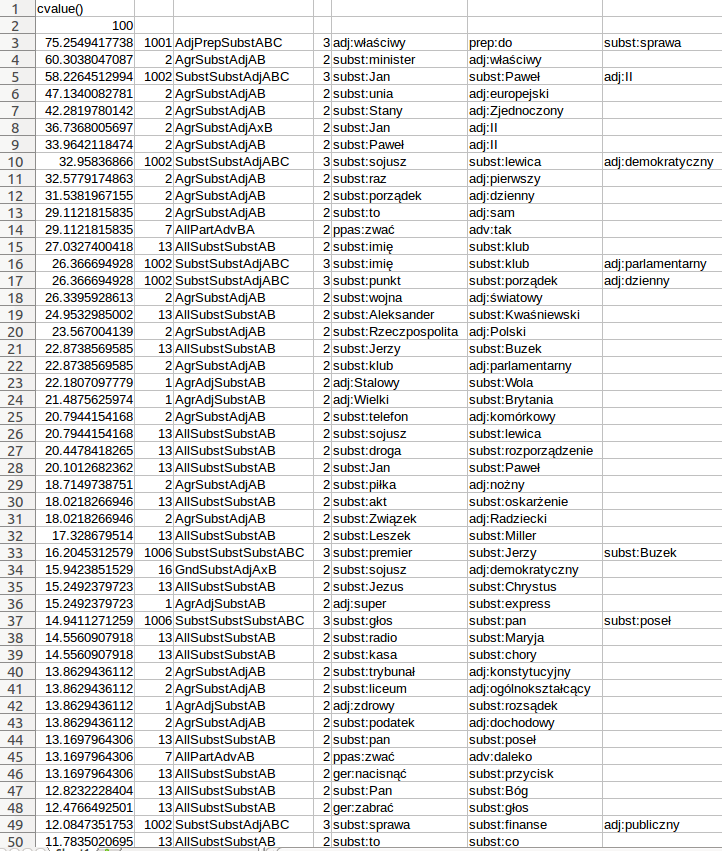
\includegraphics[scale=0.45]{img/cval_res.png}
    \caption{Results obtained with use of C-value association measure}
    \label{img_cval}
\end{figure}
